\documentclass[letterpaper, 10 pt, conference]{ieeeconf}

% numbers option provides compact numerical references in the text. 
\usepackage{times}
\usepackage{acronym}
\usepackage{xcolor, graphicx}
\usepackage{float}
\usepackage{caption}
\usepackage[utf8]{inputenc} 
\usepackage{multicol}
\usepackage{cite}
\usepackage{amsmath}
\usepackage{mathtools}
\usepackage[bookmarks=true]{hyperref}
\usepackage{multirow}
\usepackage{arydshln}
\usepackage{subcaption}

\pdfinfo{
   /Author (Miguel Faria)
   /Title  (Understanding Robots - Making Robots More Legible in Multi-User Interactions)
   /CreationDate (D:20200228)
   /Subject (Robotic Communication)
   /Keywords (Robots; Robotic Communication; Legibility; Multi-User Interaction)
}

\IEEEoverridecommandlockouts
\overrideIEEEmargins

\DeclareMathOperator*{\argmax}{arg\,max}
\newcommand{\norm}[1]{\left\lVert#1\right\rVert}

\begin{document}

% paper title
\title{\LARGE \bf
Understanding Robots - Making Robots More Legible in Multi-User Interactions
}


\author{Miguel Faria$^{1}$ \and Francisco S. Melo$^{1}$ \and Ana Paiva$^{1}$% <-this % stops a space
%\thanks{*This work was not supported by any organization}% <-this % stops a space
\thanks{$^{1}$ All authors are with INESC-ID and Instituto Superior T\'{e}cnico, University of Lisbon, Portugal. E-mail:
        {\tt\small miguel.faria@tecnico.ulisboa.pt} and {\tt\small\{fmelo,ana.paiva\}@inesc-id.pt}.}%
}

% You will get a Paper-ID when submitting a pdf file to the conference system
% \author{Author Names Omitted for Anonymous Review. Paper-ID [add your ID here]}

%\author{\authorblockN{Michael Shell}
%\authorblockA{School of Electrical and\\Computer Engineering\\
%Georgia Institute of Technology\\
%Atlanta, Georgia 30332--0250\\
%Email: mshell@ece.gatech.edu}
%\and
%\authorblockN{Homer Simpson}
%\authorblockA{Twentieth Century Fox\\
%Springfield, USA\\
%Email: homer@thesimpsons.com}
%\and
%\authorblockN{James Kirk\\ and Montgomery Scott}
%\authorblockA{Starfleet Academy\\
%San Francisco, California 96678-2391\\
%Telephone: (800) 555--1212\\
%Fax: (888) 555--1212}}


% avoiding spaces at the end of the author lines is not a problem with
% conference papers because we don't use \thanks or \IEEEmembership


% for over three affiliations, or if they all won't fit within the width
% of the page, use this alternative format:
% 
%\author{\authorblockN{Michael Shell\authorrefmark{1},
%Homer Simpson\authorrefmark{2},
%James Kirk\authorrefmark{3}, 
%Montgomery Scott\authorrefmark{3} and
%Eldon Tyrell\authorrefmark{4}}
%\authorblockA{\authorrefmark{1}School of Electrical and Computer Engineering\\
%Georgia Institute of Technology,
%Atlanta, Georgia 30332--0250\\ Email: mshell@ece.gatech.edu}
%\authorblockA{\authorrefmark{2}Twentieth Century Fox, Springfield, USA\\
%Email: homer@thesimpsons.com}
%\authorblockA{\authorrefmark{3}Starfleet Academy, San Francisco, California 96678-2391\\
%Telephone: (800) 555--1212, Fax: (888) 555--1212}
%\authorblockA{\authorrefmark{4}Tyrell Inc., 123 Replicant Street, Los Angeles, California 90210--4321}}

\maketitle

\begin{abstract}
Robots need to correctly communicate to be fully integrated in society. This communication happens in a different ways, some more explicit like when we talk and others more implicit that require interpretation as happens with facial expression. In this work we explore one way of implicit communication - movement - in multi-user interactions and how can a robot move to better communicate its intentions using legible movement.

Most research into legibility in robotics focus on single-user interactions, exploring various factors than can impact the legibility of a movement such as a user's point-of-view or how a user reacts when faced with a robot using legible movements. In this work we tackle another factor that impacts legibility, the number of humans the robot has to interact with simultaneously. We propose and validate an extension to how legible movements are generated for a robot that takes into account the various humans' different points-of-view in both the evaluation and generation of legible movements. We propose that the legibility metric is an average of the legibilities for all human partners, taking into consideration how all of them perceive a movement from their respective points-of-view.

We show, through a user study and simulations, that our proposed model o Multi-User Legibility creates movements that, although do not optimize each human's legibility, on average optimize the legibility of the group. Generating movements that allow each human interacting more quickly and confidently understand what the robot's intentions, creating safer, clearer and more efficient interactions and collaborations.
\end{abstract}

\IEEEpeerreviewmaketitle

\section{Introduction}
\label{sec:introduction}

Robots are an increasingly more common sight in everyday lives in the most diverse capabilities, from toys like Anki's Vector to iRobot's Roomba vaccum cleaner to Paro the Therapeutic Robot. Thus, research in the field human-robot interaction and its possible applications has been important for a correct integration of robots and adapting them to correctly assist in tasks like healthcare\cite{melo2019aim, kaplan2016icra, huijnen2016jadd}, education\cite{chandra2016roman, yadollahi2018cidc}, entertainment\cite{correia2017social}, amongst others. However, to fully integrate robots in society, they need to be able to correctly interact and communicate with humans. The need for correct communication is essential for interactions between humans and robots to be safe\cite{michalos2015cirp}, natural\cite{sauppe2014sigchi} and efficient. \cite{mutlu2013hri, goodrich2003smc}

Humans communicate in a myriad of different ways: some explicitly convey intention, like speech or haptic communication; others implicitly convey intention, like body movements or proactively executing an action or task, requiring interpretation by the receiver on the sender's intentions. \cite{bauer2008ijhr} The combination of explicit and implicit communication allows humans to easily interact with each other, even in situations where no explicit signals are traded. Like collaborative tasks, where all parties work together towards the same goal without always explicitly communicating their current objectives or intentions. Robots involved in human-robot interactions must then also leverage explicit and implicit means of communication for those interactions to feel normal by humans. Thus, taking advantage of the humans' natural inclination to resort to implicit communication cues to help in understanding intentions. \cite{gildert2018frontiers} 

In fact, leveraging both implicit and explicit communication has been shown to have positive impacts in human-robot interactions. Breazeal et al.\cite{breazeal2005iros} showed how the use of a combination of implicit and explicit communication, in a collaborative task, caused less errors and less time to finish the task in than using only explicit communication. Likewise, in \cite{liang2019chi}, Liang et al. applied an AI agent that used implicature - an implicit communication where utterances imply information beyond that the words literally convey - in a collaborative game achieving more natural-like interactions. In \cite{faria2016roman, baraka2016expressive} robots used signaling and body movements to convey intentions, thus overcoming limitations caused by their embodiment.

Nonverbal communication through movement is an essential mean of implicit communication, because it is cross-cultural and most humans comprehend without being previously explicitly taught. \cite{ekman1969repertoire} The use body movement by a robot can lead to people considering it more socially engaging, warm, friendly and empathetic; as well as more expressive when conveying different emotions. The correct use of body movement can also improve task performance, causing less errors and better completion times. \cite{saunderson2019ijsr} Both \cite{dragan2015hri, faria2017iros} use expressive movements, called legible movements, to allow the human partners to better understand the robot's objectives. In \cite{faria2016roman}, expressive movements mimicking those of home pets improved a Sphero robot communication capabilities, allowing humans to understand they should follow the robot to another room. Che et al. \cite{che2020tr}, combined explicit communication and body movements to make a robotic mobile platform navigate through an environment shared with humans without colliding with humans and reduce human effort in predicting the robot's intentions.

Legible movements, defined by Dragan et al. in \cite{dragan2013hri}, are movements that augment a robot's expressiveness by making their movements easier to read by users through an exaggeration of the robot's trajectory that removes doubt about what the robot is reaching for or what its objective is. Legible movements have been explored to understand their true impacts and advantages in human-robot interactions. In \cite{dragan2015hri, faria2017iros}, legible movement was explored as a means to improve the efficiency of a team in human-robot collaboration tasks. Busch et al. \cite{busch2017ijsr} explored how a robot can improve it's legibility by learning while interacting with humans to improve their prediction capabilities regarding the robot's objectives. Legible motion is also powerful because it increases the transparency of a robot's state, as evidenced in \cite{kwon2018hri} where a robot used legible movements to express its limitations and incapabilities.

Most works explore the uses and capabilities of legible movements in single-user scenarios \cite{dragan2015hri, busch2017ijsr}. However, when integrated in society, a robot must be expressive both in single and multi-user scenarios, as would happen in a surgery scenario \cite{kaplan2016icra}, or in an educational scenario where a robot would has to interact with multiple learners. Given evidences that support the use of legible movement in multi-user scenarios for specific tasks \cite{faria2017iros}, we find necessary to explore how legible movements would impact multi-user interactions

In this work we propose an extension to how we have looked at legibility and how to generate legible movements. We propose generating legibility by evaluating the legibility of the movement as the average legibility for all partners involved in the task or interaction, instead of individually evaluating the legibility of a movement for each partner. By considering the average of the legibilities, the movement will be legible for all partners, instead of possibly legible for one but not legible for the other partners.

In the following sections we will, in section \ref{sec:legibility}, define what are legible movements and the principles behind legibility, as well as how to create legible movements considering each person's \ac{POV}. In section \ref{sec:multi-user-legibility} we will explore how to consider legibility in multi-user scenarios, the drawbacks of considering only single users and how to generate legible movements that take into consideration multiple users. In section \ref{sec:experiments}, we will show the results of the two different validations: a simulation test that compares the legibility of the multi-user approach versus the traditional single-user approach in a multi-user interaction scenario in section \ref{subsec:simulations} and in section \ref{subsec:user-study} the results of the user study conducted on \ac{M-Turk}, using the same scenario as in section \ref{subsec:simulations}.

%%%%%%%%%%%%%%%%%%%%%%%%%%%%%%%%%%%%%%%%%%%%%%%%%%%%%%%%%%%%%%%%%%%%%%%%%%%%%%%%%%

\section{Legible Motion}
\label{sec:legibility}

% Definition of legible motion according to Dragan et al. 2013
Legible motion was presented by Dragan et al. in \cite{dragan2013hri} as type of movement that allowed a robot to be more expressive during interaction with humans, drawing on the fact that humans interpret an action's objective in a \emph{goal-oriented} manner. \cite{csibra2007ap} This means that humans, when observing an agent performing an action, they consider the agent to be logical and thus will execute the action in the most efficient way possible. Leveraging on this fact, a legible movement tries emphasize the movement's objective by performing a movement that brings the robot as close as possible to the objective and at the same time as far away as possible from other possible objectives as soon as possible.

To achieve this emphasis on the objective, legible movements leverage animation principles to create trajectories that are readable\cite{takayama2011hri} and that encourage "anticipatory"\cite{gielniak2013ijrr} movements, creating trajectories that convey the most relevant information for goal prediction in the beginning of the movement. A legible movement is then a movement that, when observed by a human, allows the human to infer the objective $G_R$ as soon as possible given the observed movement $\xi$:

%
\begin{equation}
    \label{eq:1}
	Legibility(\xi) = \frac{\int P(G_R|\xi_{S\to\xi(t)})f(t)dt}{\int f(t) dt},
\end{equation}
%

where $P(G_R|\xi_{S\to\xi(t)})$ is the probability of achieving objective $G_R$ given the observed trajectory $\xi_{S\to \xi(t)}$. The term $P(G_R|\xi_{S\to\xi(t)})$ in equation \ref{eq:1} models how a human attributes the probability of the goal $G_R$ being reached by trajectory $\xi$ observed until timestep $t$.\cite{dragan2013hri} The cost function used in $C(x)$ models how a human expects the robot to move in an efficient manner, with lower costs meaning more efficient and predictable trajectories. Following previous works as \cite{dragan2013generating}, one possible cost function is the sum of squared velocities $C(\xi) = \frac{1}{2} \int{\norm{\xi'(t)}^2}$ that encourages smooth trajectories that go straight to the goal.

Using the definition of legibility in equation \ref{eq:1}, it is possible to generate legible trajectories using a gradient ascent approach that in each iteration improves the legibility score of the trajectory $\xi$:

\begin{equation}
    \label{eq:3}
	\xi_{i+1} = \xi_i + \frac{1}{\eta} M^{-1} \nabla Legibility(\xi),
\end{equation}

$M$ is used to measure the norm of a trajectory, $\norm{\xi}^2_A = \xi^T A \xi$.

% Improvement with viewpoint legibility in Nikoladis et al. 2016
Legible movement as \cite{dragan2013hri} assumes humans have an omniscient view workspace. This assumption can lead to movements that go outside the \ac{FOV} of a human, passes through human blind spots or through obstructed parts of the workspace, creating trajectories that are not as legible as expected. To solve this problem, Nikoladis et al. in \cite{nikolaidis2016hri} propose an extension to the original approach where the cost function $C(x)$ becomes a function $\overline{C}(x) = C(\overline{\xi}) = C(T(\xi))$, with $T(\xi)$ a transformation that combines the transformation of trajectory $\xi$ from world coordinates to the human referential and then projects the 3D points into 2D points in the human \ac{FOV}.

With the extension, the legibility metric loses the omniscient approach and instead the trajectory is projected to the human \ac{FOV} before calculating the legibility of the trajectory. The transformation into the human's viewpoint allows the optimization procedure to improve the legibility of the trajectory creating trajectories that are always inside the user's \ac{FOV}. This improves the human partner's ability to correctly predict the robot's objective. \cite{nikolaidis2016hri} We will refer to this as \textbf{\ac{SUL}}.

%%%%%%%%%%%%%%%%%%%%%%%%%%%%%%%%%%%%%%%%%%%%%%%%%%%%%%%%%%%%%%%%%%%%%%%%%%%%%%%%%%

\section{Multi-User Legible Motion}
\label{sec:multi-user-legibility}

As addressed in section \ref{sec:legibility}, legible motions were defined to allow robots to be more expressive by leveraging the human rational thinking of an agent's action and animation principals to create movements that convey intentions as soon as possible. These motions have been tested in single-user scenarios: scenarios where a robot interacts with one human at a time. However, there are several example of scenarios where a robot must interact with multiple humans at the same time. Examples of these are \cite{correia2017social} where a robot plays a game of cards with three other people; \cite{kaplan2016icra} where a robot would be inserted in a surgical team to support the staff; or \cite{faria2017iros} where a robot has to sequentially fill cups of water to different human partners. In all of these scenarios, for a robot to use legible motions it must be able to generate movements that are simultaneously legible for all partners involved, otherwise it could optimize the legibility for one partner but reduce the legibility for another one, if that partner's view of the workspace is not adequate.

For legible motions to be legible to multiple users simultaneously, we propose an extension to \ac{SUL} where instead of the legibility metric only consider one user, it will equally consider all users when evaluating the legibility of a trajectory. We propose the legibility metric be an average of the legibilities for each user. So, when we improve the legibility we are creating a trajectory that is not perfect for one partner, but instead maximizes the average legibility of the group. We this humans can better understand the robot, leading to better cooperation within the group. We name this new approach to legibility \textbf{\ac{MUL}}.

\subsection{Definition of Multi-User Legibility}
\label{subsec:multi-user-legibility-math}

In \ac{MUL}, we define the legibility of a trajectory $\xi$ as follows:
%
\begin{equation}
    \label{eq:4}
    Legibility_{MUL}(\xi) =  \frac{ \sum_{n=1}^{N} Legibility_{SUL_n}(\xi)}{N},
\end{equation}
%
where $N$ is the number of human partners and $Legibility_{SUL_n}(\xi)$ is the legibility of the trajectory $\xi$ for one of the human partners, i.e., the legibility of the trajectory in the \ac{POV} of one of the human partners as in \ac{SUL}.

With \ac{MUL} the expression for the update in optimization procedure becomes
%
\begin{equation}
    \label{eq:5}
    \xi_{i+1} = \xi_i + \frac{1}{\eta} M^{-1} \nabla Legibility_{MUL}(\xi),
\end{equation}
%
with 
%
\begin{equation}
    \label{eq:6}
    \nabla Legibility_{MUL}(\xi) = \frac{ \sum_{n=1}^{N} T_n^{-1} \cdot \nabla Legibility_{SUL_n}(\xi)}{N},
\end{equation}
%
where $T_n^-1$ is the transformation from the human partner to the coordinate space where $\xi$ was defined and
%
\begin{equation}
    \label{eq:7}
    \nabla Legibility_{SUL_n}(\xi) = \nabla \mathcal{L}(\xi(t)) \cdot \nabla_{3D}^{2D} T_n(\xi(t)),
\end{equation}
%
where $\nabla \mathcal{L}(\xi(t))$ is as defined in \cite{dragan2013generating} and $\nabla_{3D}^{2D} T_(\xi(t))$ is the gradient for the transformation of the trajectory $\xi$ to the perspective of the human partner in question.

%%%%%%%%%%%%%%%%%%%%%%%%%%%%%%%%%%%%%%%%%%%%%%%%%%%%%%%%%%%%%%%%%%%%%%%%%%%%%%%%%%

\section{Model applied}
\label{sec:experiments}

We validated our proposed model in two stages: first we defined a simulation scenario where we compared the legibility of a trajectory optimized using \ac{MUL}, versus the average legibility of trajectories that used \ac{SUL}; second, we used the same scenario, created videos for trajectories executed by a robot using \ac{MUL} and \ac{SUL} and tested how the trajectories obtained differed for real humans.

\subsection{Simulations}
\label{subsec:simulations}

% Define simulation environment
The scenario for the simulations was an interaction where a robot had to grab one of three objects on a table - a soda can, a rubber duck and a telephone - and three humans had to predict which object the robot was going to grab. We defined four different configurations of object positioning and human poses, under the restriction that the human orientation was such that their \ac{FOV} captured both the robot and the objects on the table. Also, since we were modeling a real world scenario, the human were oriented as if looking in a slightly downward manner as they would in real life; this downward angle would vary between $10º$ and $15º$ depending on the distance between the human and the objects on the table. The different configurations are showed in Figure \ref{fig:simulation-configurations} and represent configurations of objects that one could face in real world interactions with the robot.

For each configuration, we ran four optimizations on legibility - one using \ac{MUL} and one using \ac{SUL} applied to each of the defined points of view - starting with a straight line from the robot's starting position to the target of the optimization - one of the soda can, rubber duck or telephone. The optimization process stopped either when the maximum number of iterations was reached or if the difference between improvements was less than a defined threshold. After each optimization finished, we evaluated the obtained trajectory's legibility for each user. 

\begin{figure}[t]
    \centering
    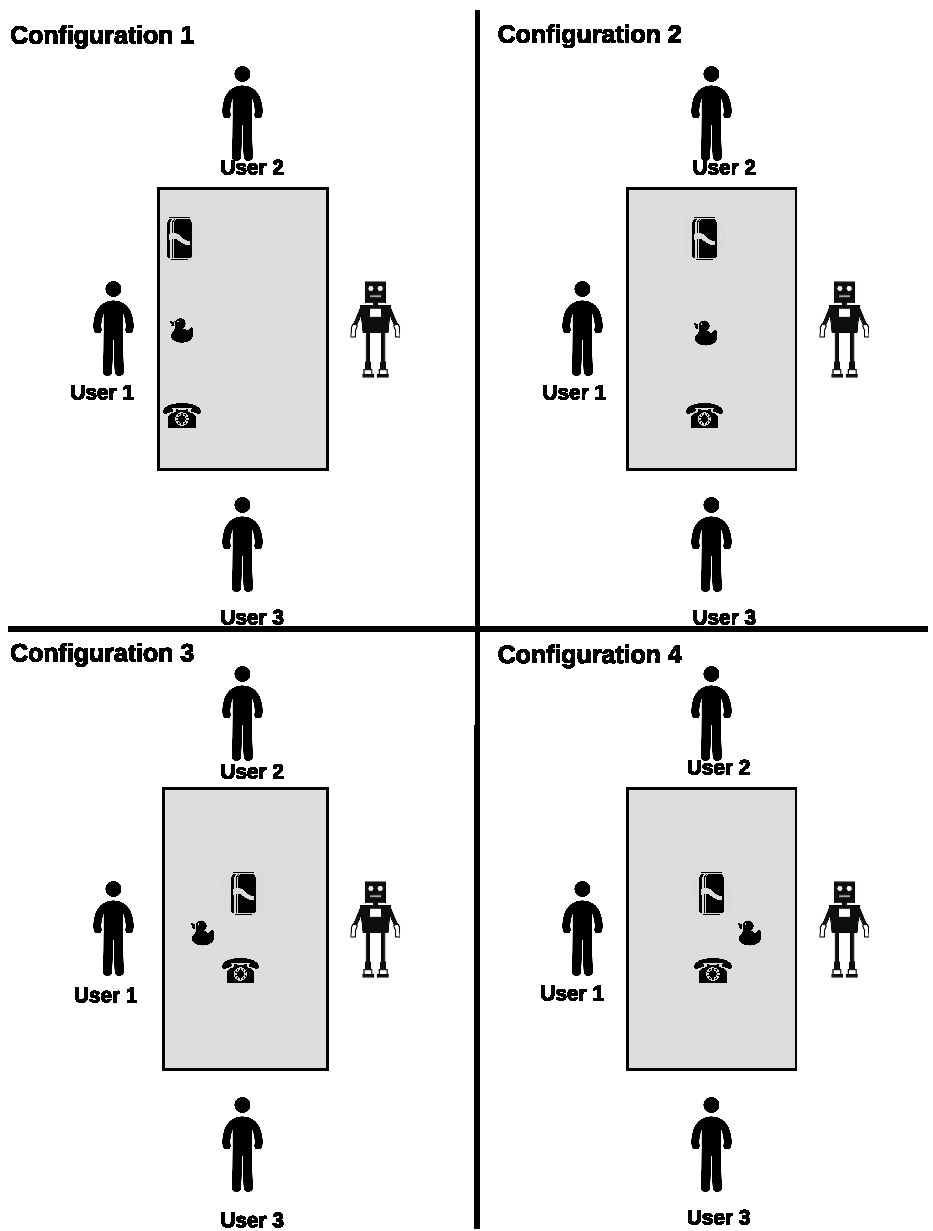
\includegraphics[width=.9\linewidth, height=6cm]{images/simulation_configurations.pdf}
    \caption{The different configurations of the targets - soda can, rubber duck and telephone - and users - User 1 opposite to the robot, User 2 to the right of the robot and User 3 to the left of the robot. The configurations presented are numbered from configuration 1 in the top left corner to configuration 4 in the bottom right.}
    \label{fig:simulation-configurations}
\end{figure}


% Simulation results
\subsubsection{\textbf{Results and Analysis}}
Tables \ref{tab:sim-results-a}, \ref{tab:sim-results-b}, \ref{tab:sim-results-c} present the results for the simulations. Each table presents the legibility results for one of the three targets: table \ref{tab:sim-results-a} the soda can, table \ref{tab:sim-results-b} the rubber duck and table \ref{tab:sim-results-c} the telephone; organized by the configuration and the optimization applied - either optimized using \ac{MUL} or with \ac{SUL} for each user. When evaluating the trajectory's legibility for each user, if the trajectory would pass outside a user's \ac{FOV} it was attributed a legibility value 0. This attribution was based on the fact that trajectories outside the \ac{FOV} can lead to unsafe and harmful interactions and an incorrect communication of intentions.

\begin{table}[]
\begin{tabular}{|cc|c|c|c|c|}
\hline
                                         &         & \multicolumn{4}{c|}{Optimization}       \\ \hline
\multicolumn{1}{|c|}{}                   &         & \ac{MUL} & \ac{SUL} User 1 & \ac{SUL}  User 2 & \ac{SUL} User 3 \\ \hline
\multicolumn{1}{|c|}{\multirow{4}{*}{1}} & User 1  & 0.86698   & 0.85394 & 0.48204 & 0       \\ \cdashline{2-6} 
\multicolumn{1}{|c|}{}                   & User 2  & 0.93454   & 0       & 0.59744 & 0       \\ \cdashline{2-6} 
\multicolumn{1}{|c|}{}                   & User 3  & 0.862486  & 0.84119 & 0.45229 & 0.93651 \\ \cdashline{2-6} 
\multicolumn{1}{|c|}{}                   & Average & 0.888     & 0.56504 & 0.51059 & 0.31217 \\ \hline
\multicolumn{1}{|c|}{\multirow{4}{*}{2}} & User 1  & 0.46814   & 0.58293 & 0.27584 & 0.73607 \\ \cdashline{2-6} 
\multicolumn{1}{|c|}{}                   & User 2  & 0.51256   & 0.87007 & 0.8644  & 0       \\ \cdashline{2-6} 
\multicolumn{1}{|c|}{}                   & User 3  & 0.59155   & 0.67691 & 0.03682 & 0.93358 \\ \cdashline{2-6} 
\multicolumn{1}{|c|}{}                   & Average & 0.52408   & 0.70997 & 0.39235 & 0.55655 \\ \hline
\multicolumn{1}{|c|}{\multirow{4}{*}{3}} & User 1  & 0.57381   & 0.87294 & 0.31076 & 0.55507 \\ \cdashline{2-6} 
\multicolumn{1}{|c|}{}                   & User 2  & 0.33217   & 0       & 0.83371 & 0.03175 \\ \cdashline{2-6} 
\multicolumn{1}{|c|}{}                   & User 3  & 0.8118    & 0.93651 & 0.0331  & 0.93651 \\ \cdashline{2-6} 
\multicolumn{1}{|c|}{}                   & Average & 0.57259   & 0.60315 & 0.39252 & 0.50777 \\ \hline
\multicolumn{1}{|c|}{\multirow{4}{*}{4}} & User 1  & 0.48004   &         & 0.43542 & 0.03194 \\ \cdashline{2-6} 
\multicolumn{1}{|c|}{}                   & User 2  & 0.90923   &         & 0.50269 & 0       \\ \cdashline{2-6} 
\multicolumn{1}{|c|}{}                   & User 3  & 0.52480   &         & 0.40403 & 0.92770 \\ \cdashline{2-6} 
\multicolumn{1}{|c|}{}                   & Average & 0.63803   &         & 0.44738 & 0.31988 \\ \hline
\end{tabular}
\caption{Table with the resulting legibility values for each user and the users' average, given one of the configurations in Figure \ref{fig:simulation-configurations} and the optimization used, for the soda can.}
\label{tab:sim-results-a}
\end{table}


\begin{table}[]
\begin{tabular}{|cc|c|c|c|c|}
\hline
                                         &         & \multicolumn{4}{c|}{Optimization}       \\ \hline
\multicolumn{1}{|c|}{}                   &         & \ac{MUL} & \ac{SUL} User 1 & \ac{SUL}  User 2 & \ac{SUL} User 3 \\ \hline
\multicolumn{1}{|c|}{\multirow{4}{*}{1}} & User 1  & 0.56878   & 0.56795 & 0.56315 & 0.56315 \\ \cdashline{2-6} 
\multicolumn{1}{|c|}{}                   & User 2  & 0.47615   & 0.47969 & 0.48196 & 0.46095 \\ \cdashline{2-6} 
\multicolumn{1}{|c|}{}                   & User 3  & 0.47615   & 0.47969 & 0.46095 & 0.48196 \\ \cdashline{2-6} 
\multicolumn{1}{|c|}{}                   & Average & 0.50703   & 0.50911 & 0.50202 & 0.50202 \\ \hline
\multicolumn{1}{|c|}{\multirow{4}{*}{2}} & User 1  & 0.36148   & 0.3615  & 0.36147 & 0.36147 \\ \cdashline{2-6} 
\multicolumn{1}{|c|}{}                   & User 2  & 0.38534   & 0.3853  & 0.38535 & 0.38532 \\ \cdashline{2-6} 
\multicolumn{1}{|c|}{}                   & User 3  & 0.38534   & 0.3853  & 0.38532 & 0.38535 \\ \cdashline{2-6} 
\multicolumn{1}{|c|}{}                   & Average & 0.37738   & 0.37737 & 0.37738 & 0.37738 \\ \hline
\multicolumn{1}{|c|}{\multirow{4}{*}{3}} & User 1  & 0.57381   & 0.87294 & 0.55507 & 0.31076 \\ \cdashline{2-6} 
\multicolumn{1}{|c|}{}                   & User 2  & 0.8118    & 0.93651 & 0.9365  & 0.0331  \\ \cdashline{2-6} 
\multicolumn{1}{|c|}{}                   & User 3  & 0.33217   & 0       & 0.03175 & 0.83371 \\ \cdashline{2-6} 
\multicolumn{1}{|c|}{}                   & Average & 0.57259   & 0.60315 & 0.50777 & 0.39252 \\ \hline
\multicolumn{1}{|c|}{\multirow{4}{*}{4}} & User 1  &           &         &         &         \\ \cdashline{2-6} 
\multicolumn{1}{|c|}{}                   & User 2  &           &         &         &         \\ \cdashline{2-6} 
\multicolumn{1}{|c|}{}                   & User 3  &           &         &         &         \\ \cdashline{2-6} 
\multicolumn{1}{|c|}{}                   & Average &           &         &         &         \\ \hline
\end{tabular}
\caption{Table with the resulting legibility values for each user and the users' average, given one of the configurations in Figure \ref{fig:simulation-configurations} and the optimization used, for the rubber duck.}
\label{tab:sim-results-b}
\end{table}

\begin{table}[]
\begin{tabular}{|cc|c|c|c|c|}
\hline
                                         &         & \multicolumn{4}{c|}{Optimization}       \\ \hline
\multicolumn{1}{|c|}{}                   &         & \ac{MUL} & \ac{SUL} User 1 & \ac{SUL}  User 2 & \ac{SUL} User 3 \\ \hline
\multicolumn{1}{|c|}{\multirow{4}{*}{1}} & User 1  & 0.86698   & 0.85082 & 0       & 0.48324 \\ \cdashline{2-6} 
\multicolumn{1}{|c|}{}                   & User 2  & 0.86249   & 0.84132 & 0.93651 & 0.47535 \\ \cdashline{2-6} 
\multicolumn{1}{|c|}{}                   & User 3  & 0.93454   & 0       & 0       & 0.58933 \\ \cdashline{2-6} 
\multicolumn{1}{|c|}{}                   & Average & 0.888     & 0.56405 & 0.31217 & 0.51597 \\ \hline
\multicolumn{1}{|c|}{\multirow{4}{*}{2}} & User 1  & 0.46814   & 0.75825 & 0.7569  & 0.26634 \\ \cdashline{2-6} 
\multicolumn{1}{|c|}{}                   & User 2  & 0.59155   & 0.8486  & 0.93482 & 0.03186 \\ \cdashline{2-6} 
\multicolumn{1}{|c|}{}                   & User 3  & 0.51257   & 0       & 0       & 0.93414 \\ \cdashline{2-6} 
\multicolumn{1}{|c|}{}                   & Average & 0.52408   & 0.53562 & 0.56391 & 0.41078 \\ \hline
\multicolumn{1}{|c|}{\multirow{4}{*}{3}} & User 1  & 0.81781   & 0.65822 & 0.93334 & 0.93334 \\ \cdashline{2-6} 
\multicolumn{1}{|c|}{}                   & User 2  & 0.36397   & 0.36358 & 0.45865 & 0.3339  \\ \cdashline{2-6} 
\multicolumn{1}{|c|}{}                   & User 3  & 0.36397   & 0.36358 & 0.3339  & 0.45865 \\ \cdashline{2-6} 
\multicolumn{1}{|c|}{}                   & Average & 0.51525   & 0.4618  & 0.5753  & 0.5753  \\ \hline
\multicolumn{1}{|c|}{\multirow{4}{*}{4}} & User 1  &           &         &         &         \\ \cdashline{2-6} 
\multicolumn{1}{|c|}{}                   & User 2  &           &         &         &         \\ \cdashline{2-6} 
\multicolumn{1}{|c|}{}                   & User 3  &           &         &         &         \\ \cdashline{2-6} 
\multicolumn{1}{|c|}{}                   & Average &           &         &         &         \\ \hline
\end{tabular}
\caption{Table with the resulting legibility values for each user and the users' average, given one of the configurations in Figure \ref{fig:simulation-configurations} and the optimization used, for the telephone.}
\label{tab:sim-results-c}
\end{table}

% Analysis of results
The legibility values in tables \ref{tab:sim-results-a}, \ref{tab:sim-results-b}, \ref{tab:sim-results-c} show that \ac{MUL} generates trajectories that on average more legible for the entire group than if we optimize using \ac{SUL} applied to each human partner. Also, several optimizations using \ac{SUL} created trajectories that would go outside the other partners' \ac{FOV}; like in the case of the \ac{SUL} optimization for User 2 in configuration 1 for the telephone that created a trajectory with 0 legibility for both users 1 and 3. Sometimes \ac{SUL} can create trajectories that are better for the team than \ac{MUL}. This is possible if a user has a privileged perspective on the task - the human partner's \ac{FOV} gives a very good perspective on the targets and the robot - allowing \ac{SUL} to take better advantage of the \ac{POV} than \ac{MUL} because \ac{MUL} is weighted down by the other partners' \ac{POV}s. We hypothesize that possible solution to this is to give each partner a weight depending on how good a \ac{POV} is, leaving this for future work.

\subsection{User Study}
\label{subsec:user-study}

% Working hypotheses
\subsubsection{\textbf{Scenario and Hypotheses}}
We conducted a user study through \ac{M-Turk} to validate two working hypotheses:
\begin{itemize}
    \item \textbf{\emph{H1:}} Participants will consider a movement optimized using \ac{MUL} clearer than when optimized using \ac{SUL}.
    \item \textbf{\emph{H2:}} Participants will understand quicker and more confidently the robot's target, when faced with a movement optimized with \ac{MUL} than with one optimized with \ac{SUL}.
\end{itemize}

The study followed a between-subjects design, with each group being a different optimization approach - optimize for the average of all users or optimize for each user individually. Each participant watched 3 sets of 3 videos, each video with different length - 6, 12 and 18 seconds. After each video the participant was asked to predict what object the robot was going to grab and rate how confident they were in their prediction. After watching the 3 sets of videos the participant would have to rate how clear the three movements were. The videos were created using the WeBots simulator, where we recreated configuration 2 from Figure \ref{fig:simulation-configurations}.

% Results
\subsubsection{\textbf{Results and Analysis}}
We recruited 315 participants using \ac{M-Turk}, after removing those that failed the control question, with approximately 98\% from the USA and the remaining 2\% distributed across Canada, Australia and the UK. We restricted the participation on the questionnaire to these four countries to reduce language barriers problems. The participants' age varied from 23 to 76 years old and an average of 42 years old. An analysis of the education level of the participants shows that ~60\% has a higher education degree and ~90\% has finished at least high school. Regarding the occupation of the participants, 94\% are employed and ~2\% are students.

The questionnaires were analysed in two steps. The first compared the results of \ac{MUL} against each of the 3 instances of \ac{SUL}, analysing how \ac{MUL} individually fared against \ac{SUL} and the second analysis combined the results of the three applications of \ac{SUL} comparing them with \ac{MUL}, evaluating how \ac{MUL} fared against the overall performance of \ac{SUL} and attenuating the impacts of privileged and bad \ac{POV}s. For both steps we measured the average perceived clearness rate at which the participants evaluated the movements, the time taken to correctly predict the robot's target and the average confidence in the prediction. We considered that a wrong prediction of the target was considered as taking the full length of the video to make a decision and that for correct predictions the time taken corresponded to the earliest a participant answered correctly without wrongly predicting afterwards. To analyse the confidence in the prediction we combined the scores for each 6, 12 and 18 second videos as in \cite{nikolaidis2016hri}. We also conducted a normality test that showed us that all three measures - average perceived clearness, time taken and confidence - did not follow a normal distribution.

To verify hypothesis \textbf{H1}, we conducted a Kurskal-Wallis test comparing \ac{MUL} individually with all the applications of \ac{SUL} showing a significant difference between the four optimizations, $\chi^2(3)=9.344, p=0.025$. A follow-up analysis with a Mann-Whitney test to determine where this difference existed, showed that \ac{MUL} was rated as significantly clearer than the application of \ac{SUL} to User 2 ($U=2250, p=0.009$) and User 3 ($U=2333.50, p=0.008$), thus supporting hypothesis \textbf{H1} for both users. For the comparison between \ac{MUL} and the aggregated \ac{SUL} applications, we conducted a Mann-Whitney test that showed \ac{MUL} was considered significantly clearer by users than \ac{SUL}, $U=7277.5, p=0.006$, thus supporting hypothesis \textbf{H1}. Figure \ref{fig:results-clearness} shows the result distribution of perceived clearness for both analysis: the individual on the left graph and the aggregated on the right graph, with the average for each mark with a point.

\begin{figure*}[t]
  \begin{subfigure}[b]{0.5\textwidth}
    \centering
    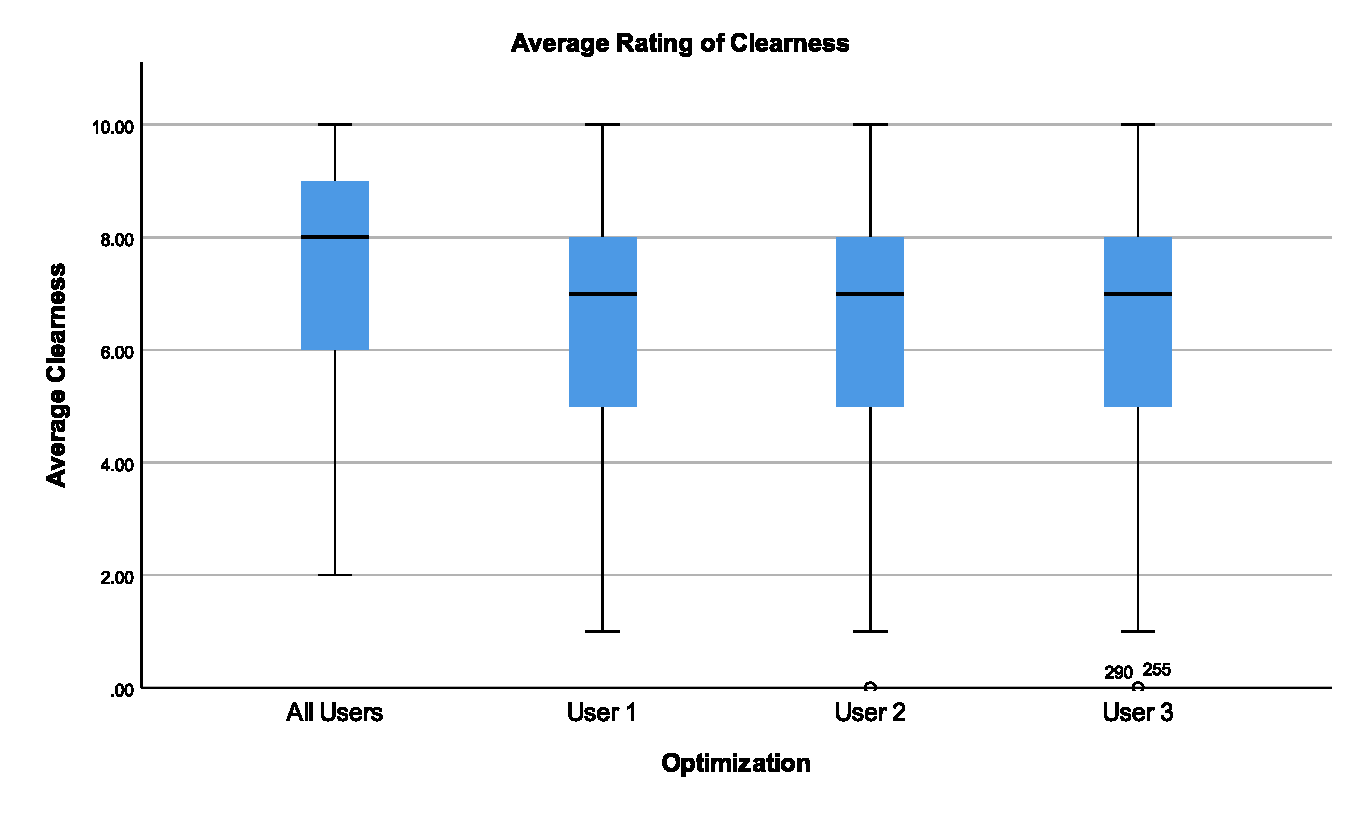
\includegraphics[width=\linewidth, height=4cm]{images/multi-user-legibility-study-clearness-graph}
    \caption{}
    \label{fig:results-clearness}
  \end{subfigure}
  \hfill %%
  \begin{subfigure}[b]{0.5\textwidth}
    \centering
    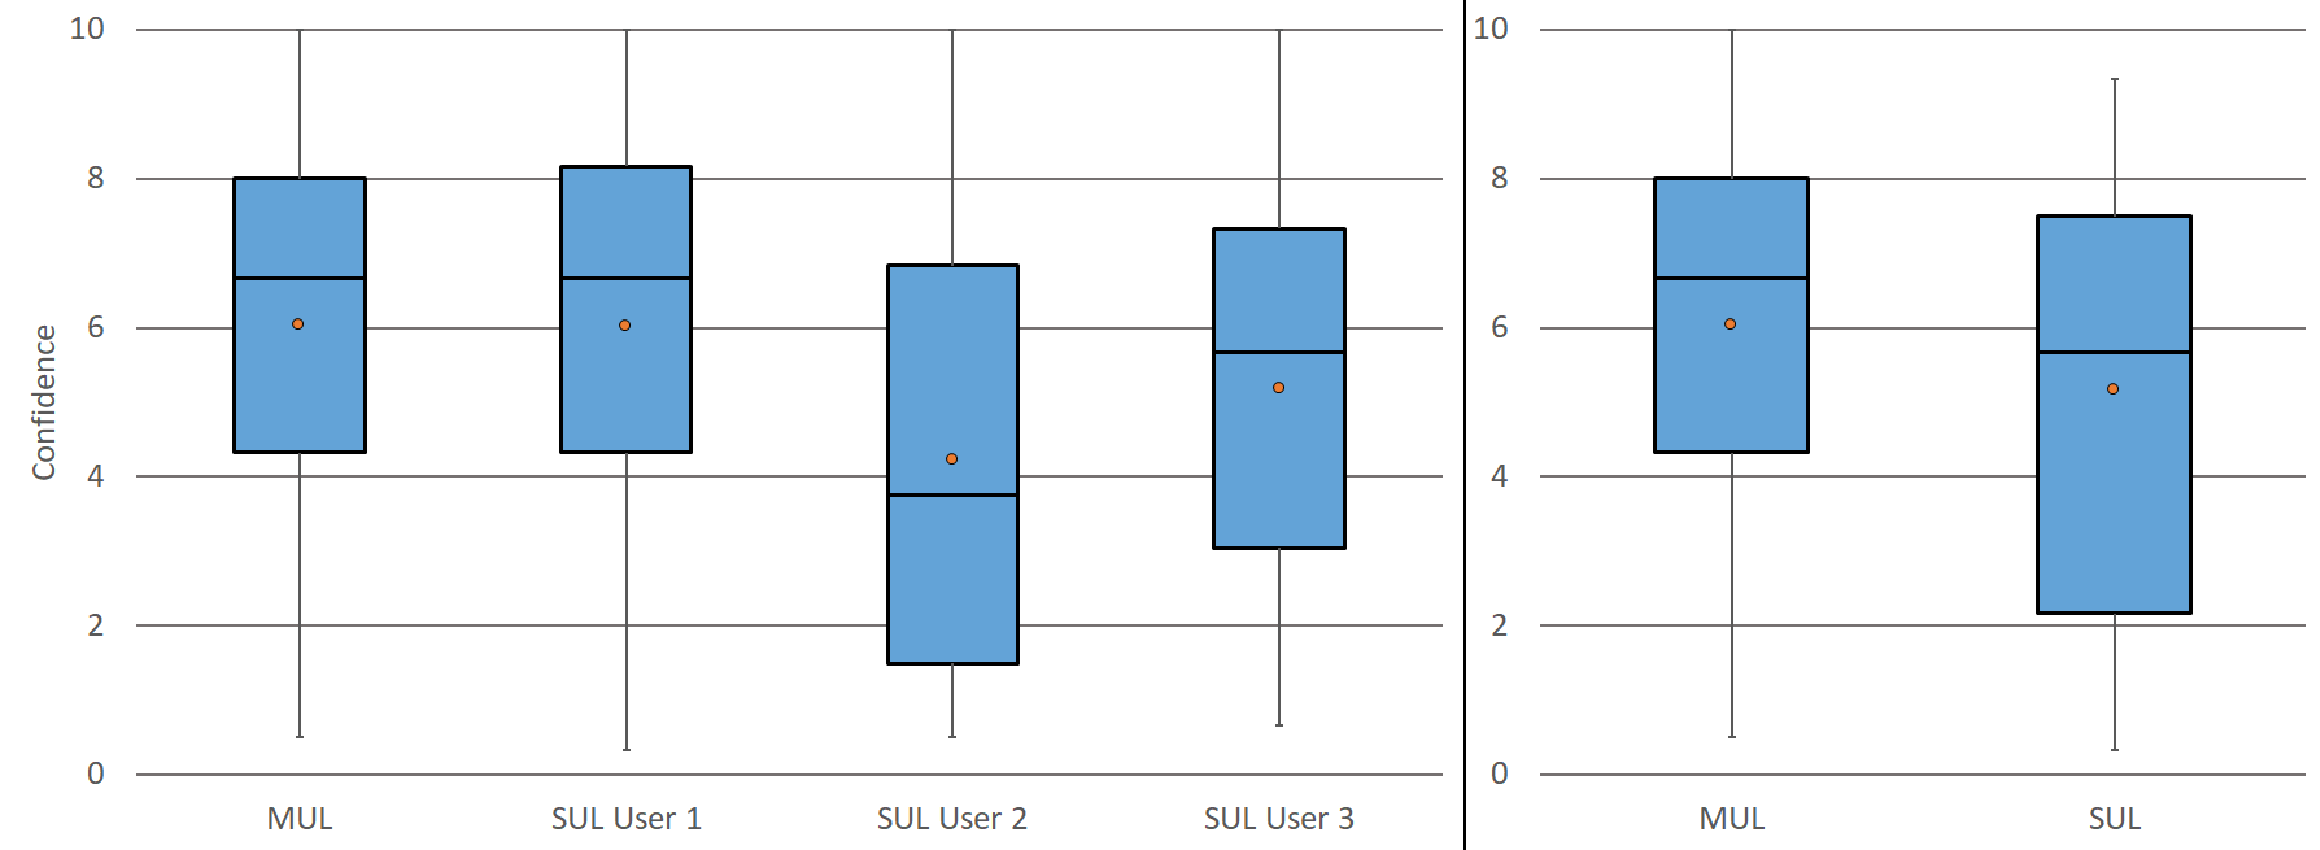
\includegraphics[width=\linewidth, height=4cm]{images/multi-user-legibility-study-confidence-graph}
    \caption{}
    \label{fig:results-confidence}
  \end{subfigure}
  \caption{Box plots comparing the distributions and average values for perceived clearness and confidence in predictions. Figure \ref{fig:results-clearness} show the results for perceived clearness and Figure \ref{fig:results-confidence} the results for confidence in predictions.}
  \label{fig:results-clearness-confidence}
\end{figure*}

For hypothesis \textbf{H2}, we analysed both the time taken to predict what target the robot was going to grab and the confidence associated with said prediction. Again, both measures did not follow a normal distribution so we a applied the non-parametric Kurskal-Wallis test to find differences between the four optimizations. The Kurskal-Wallis test showed significant differences between the four optimizations for both the time ($\chi^2(3)=31.877, p<0.001$) and confidence measures ($\chi^2(3)=48.821, p<0.001$), supporting hypothesis \textbf{H2}. To further understand where both measures are most significant we applied a Mann-Whitney test, comparing the \ac{MUL} with each \ac{SUL}. For the time to correctly predict, we found participants paired with \ac{MUL} took significantly less time those paired with \ac{SUL} for User 2, $U=21244, p<0.001$. For the confidence in the predictions, we found that participants were significantly more confident in their predictions with \ac{MUL} than with \ac{SUL} for User 2, $U=11379, p<0.001$, and for User 3, $U=14367.5, p=0.002$, as evidenced in Figure \ref{fig:results-confidence} left graph. For the comparison between \ac{MUL} and the \ac{SUL} aggregation, we conducted a Mann-Whitney test for both the time and confidence measures. The test showed people took significantly less time to correctly predict the robot's target with \ac{MUL} optimization than with \ac{SUL} optimization, $U=75722,p=0.037$. Regarding confidence in prediction, the Mann-Whitney test and the right graph in Figure \ref{fig:results-confidence} show participants are significantly more confident in their predictions with \ac{MUL} than with \ac{SUL}, $U=43971.5,p<0.001$. Both results support hypothesis \textbf{H2}.

\section{Conclusion} 
\label{sec:conclusion}
The correct integration of robots in society requires them to be capable of correctly communicate in both single-user and multi-user interactions. In this work we presented an extension to legible movement aimed at improving robot's expressiveness in multi-user interactions, \ac{MUL}.
We showed this extension allows participants to better understand a robot's intention, creating clearer movements than the version without our extension, both in simulation and with a user study conducted through \ac{M-Turk}. The performance of \ac{MUL} is influenced by the humans' \ac{POV}s as shown by the simulation results and the differences observed in the user study between \ac{MUL} and User's 1 \ac{SUL} and \ac{MUL} and Users' 2 and 3 \ac{SUL}.

This extension is promising for its possible applications in entertainment areas such as theatre where movement are an important communication tool or healthcare in surgery teams where a robot working as part of a team needs correct communication for the rest of the medical staff correctly perform their functions.

A final aspect to highlight about \ac{MUL} is that if there is just one human interacting with the robot the model works just like \ac{SUL}.

\section*{Acknowledgments}
This work was partially supported by national funds through the Portuguese Fundação para a Ciência e a Tecnologia under project UID/CEC/50021/2013 (INESC-ID multi annual funding). Miguel Faria acknowledges the PhD grant PD/BD/143144/2019.

%% Use plainnat to work nicely with natbib. 

\bibliographystyle{IEEEtran}
\bibliography{references}

%% Acronyms definition

\acrodef{HRI}{Human-Robot Interaction}
\acrodef{SUL}{Single-User Legibility}
\acrodef{MUL}{Multi-User Legibility}
\acrodef{POV}{point-of-view}
\acrodef{FOV}{field-of-view}
\acrodef{M-Turk}{Amazon’s Mechanical Turk}

\end{document}